% This LaTeX was auto-generated from MATLAB code.
% To make changes, update the MATLAB code and export to LaTeX again.

\documentclass{article}

\usepackage[utf8]{inputenc}
\usepackage[T1]{fontenc}
\usepackage{lmodern}
\usepackage{graphicx}
\usepackage{color}
\usepackage{hyperref}
\usepackage{amsmath}
\usepackage{amsfonts}
\usepackage{epstopdf}
\usepackage[table]{xcolor}
\usepackage{matlab}

\sloppy
\epstopdfsetup{outdir=./}
\graphicspath{ {./GettingStarted_images/} }

\begin{document}

\matlabtitle{LAIIQAToolbox}

\matlabheadingthree{v1.1}

\matlabheading{Descripción}

\begin{par}
\begin{flushleft}
Programa para ajustar y graficar los datos de los archivos \texttt{.mat} generados del proceso de ozonización en el Laboratorio de Investigación en Ingeniería Química Ambiental (LAIIQA) de ESIQIE - IPN.
\end{flushleft}
\end{par}


\vspace{1em}
\begin{par}
\begin{flushleft}

\includegraphics[width=\maxwidth{56.196688409433015em}]{image_0}
\end{flushleft}
\end{par}


\vspace{1em}
\matlabheading{Requerimientos de Sistema}

\begin{par}
\begin{flushleft}
Matlab \textgreater{}= R2019.
\end{flushleft}
\end{par}

\matlabheading{Instalación}

\begin{par}
\begin{flushleft}
Desde \textbf{Add-Ons} en la pestaña \textbf{Home}, buscar como \textbf{laiiqatoolbox}.
\end{flushleft}
\end{par}

\matlabheading{Caracteristicas}

\begin{itemize}
\setlength{\itemsep}{-1ex}
   \item{\begin{flushleft} Programación orientada a objetos. \end{flushleft}}
   \item{\begin{flushleft} Grafica datos ajustados (recortados) a una concentración inicial cero (o cercana). \end{flushleft}}
   \item{\begin{flushleft} Acceso a propiedades de grafico: titulo, etiquetas de ejes \textit{x} y \textit{y, }legenda, tamaño, etc. \end{flushleft}}
   \item{\begin{flushleft} Conversión de datos de tiempo del eje \textit{x: }seg, min, h. \end{flushleft}}
   \item{\begin{flushleft} Multiselección de archivos para grafcar. \end{flushleft}}
   \item{\begin{flushleft} Acceso a variables de datos crudos (\texttt{rawdata}) y ajustados (\texttt{fixeddata}). \end{flushleft}}
   \item{\begin{flushleft} Calculo de consumo de ozono. \end{flushleft}}
   \item{\begin{flushleft} Acceso a variables de consumo de ozono (\texttt{ozoneresults}). \end{flushleft}}
   \item{\begin{flushleft} Guardado de grafico en varios formatos: png, jpg, jpeg, pdf, eps, svg, tif, fig. \end{flushleft}}
   \item{\begin{flushleft} Creación de varios objetos gráficos a la vez. \end{flushleft}}
\end{itemize}

\matlabheading{Propiedades del objeto \texttt{laiiqatoolbox}}

\begin{itemize}
\setlength{\itemsep}{-1ex}
   \item{\begin{flushleft} \texttt{rawdata: }Datos "crudos", sin tratamiento que contiene las filas de tiempo y concentración de ozono del archivo \texttt{.mat}. \end{flushleft}}
   \item{\begin{flushleft} \texttt{fixeddata: }Datos "ajustados", recortados para quitar los primeros datos de estabilización de la concentración de ozono y para comenzar el ozonograma desde una concentración igual o cercana a cero. \end{flushleft}}
   \item{\begin{flushleft} \texttt{title: }Modifica o quita el titulo del gráfico. \end{flushleft}}
   \item{\begin{flushleft} \texttt{xlabel: }Modifica los datos de tiempo. Opciones: \texttt{'seg'|} \texttt{'min'|} \texttt{'h'}. \end{flushleft}}
   \item{\begin{flushleft} \texttt{xf: }Establece el valor de \textit{x} final para cada linea de datos. Ociones: \texttt{'end'} para restaurar a todos los valores | cualquier valor positivo de tiempo. Ejemplo: \texttt{miobjeto.xf = \{ 28 'end' 45 'end' ...etc \}}. \end{flushleft}}
   \item{\begin{flushleft} \texttt{ylabel: }Cambia el titulo del eje \textit{y}. \end{flushleft}}
   \item{\begin{flushleft} \texttt{grid: }Activa o desactiva las rejillas del gráfico. Opciones: \texttt{'on'|} \texttt{'off'}. \end{flushleft}}
   \item{\begin{flushleft} \texttt{LineWidth: }Cambia el grosor de linea para todas las lineas de datos. \end{flushleft}}
   \item{\begin{flushleft} \texttt{legend: }Cambia o quita la legenda para cada linea de datos. Opciones 'default' pone de leyenda los nombres de archivos abiertos | \texttt{\{} "\textless{}nombre de leyenda 1\textgreater{}"  "\textless{}nombre de leyenda 2\textgreater{}"\texttt{  ...etc \}}. Ejemplo: \texttt{\{'default'\} }ó \texttt{\{"Linea 1" "Linea 2" "Linea 3" ...etc \}}. \end{flushleft}}
   \item{\begin{flushleft} \texttt{legendFontSize: }Cambia el tamaño de letra de todas las leyenda. \end{flushleft}}
   \item{\begin{flushleft} \texttt{legendLocation: }Ubicación de la leyenda en el gráfico. Opciones:  \texttt{'south'} | \texttt{'east'} | \texttt{'west'} | \texttt{'northeast'} | \texttt{...etc}. Ver documentación para más opciones. \end{flushleft}}
   \item{\begin{flushleft} \texttt{imageResolution: }Cambia la resolución de los formatos de imgen al guardar con el método \texttt{saveplot()}. \end{flushleft}}
   \item{\begin{flushleft} \texttt{titleInterpreter: }Interprete utilizado para el renderizado del titulo. Opciones: \texttt{'tex' (default) | 'latex'}. \end{flushleft}}
   \item{\begin{flushleft} \texttt{labelInterpreter: }Interprete utilizado para el renderizado del titulo de los ejes. Opciones: \texttt{'tex' (default) | 'latex'}. \end{flushleft}}
   \item{\begin{flushleft} \texttt{legendInterpreter: }Interprete utilizado para el renderizado de las leyedas. Opciones: \texttt{'tex' (default) | 'latex'}. \end{flushleft}}
   \item{\begin{flushleft} \texttt{ozoneUnits: }Unidades utilizadas para el cálculo del consumo de ozono. \end{flushleft}}
   \item{\begin{flushleft} \texttt{ozoneresults: }Variable que almacena los calculos del consumo de ozono. \end{flushleft}}
\end{itemize}

\matlabheading{Métodos del objeto \texttt{laiiqatoolbox}}

\begin{itemize}
\setlength{\itemsep}{-1ex}
   \item{\begin{flushleft} \texttt{openfiles: }Abre una ventana de dialogo para selececionar los archivos a graficar. \end{flushleft}}
   \item{\begin{flushleft} \texttt{plotfiles: P}rocesa los archivos seleccionados y crea el objeto gráfico. \end{flushleft}}
   \item{\begin{flushleft} \texttt{saveplot: }Guarda el objeto gráfico con el nombre y formato especificado. Ejemplo: \texttt{saveplot('nombre.pdf')}. \end{flushleft}}
   \item{\begin{flushleft} \texttt{ozonecalc: }Procesa los datos de cada archivo y calcula el ozono consumido, residual y total. \end{flushleft}}
\end{itemize}


\matlabheading{Ejemplos}


\matlabheadingtwo{Creación del objeto}

\begin{par}
\begin{flushleft}
Inicializamos una instancia de objeto de tipo \textit{\textbf{laiiqatoolbox}}:
\end{flushleft}
\end{par}

\begin{matlabcode}
clearvars
close all
clc
miobjeto1 = laiiqatoolbox
\end{matlabcode}
\begin{matlaboutput}
miobjeto1 = 
  laiiqatoolbox with properties:

              rawdata: []
            fixeddata: []
                title: "Cinética de Ozonización"
               xlabel: 'min'
                   xf: {'end'}
               ylabel: "Concentración [g/L]"
                 grid: 'on'
            LineWidth: 0.5000
               legend: {'default'}
       legendFontSize: 8
       legendLocation: 'best'
      imageResolution: 300
     titleInterpreter: 'tex'
     labelInterpreter: 'tex'
    legendInterpreter: 'tex'
           ozoneUnits: 'g/L'
         ozoneresults: []

\end{matlaboutput}


\matlabheadingtwo{Carga de archivos}

\begin{par}
\begin{flushleft}
Cargamos los archivos \textit{.mat} a graficar generados por el ozonograma con el método \texttt{openfiles}:
\end{flushleft}
\end{par}

\begin{matlabcode}
miobjeto1.openfiles
\end{matlabcode}
\begin{matlaboutput}
ans = 
  laiiqatoolbox with properties:

              rawdata: {[2x498709 double]  [2x421267 double]  [2x568493 double]}
            fixeddata: []
                title: "Cinética de Ozonización"
               xlabel: 'min'
                   xf: {'end'  'end'  'end'}
               ylabel: "Concentración [g/L]"
                 grid: 'on'
            LineWidth: 0.5000
               legend: {'default'}
       legendFontSize: 8
       legendLocation: 'best'
      imageResolution: 300
     titleInterpreter: 'tex'
     labelInterpreter: 'tex'
    legendInterpreter: 'tex'
           ozoneUnits: 'g/L'
         ozoneresults: []

\end{matlaboutput}


\matlabheadingtwo{Creación del gráfico}

\begin{par}
\begin{flushleft}
Graficamos los archivos cargados con el método \texttt{plotfiles}:
\end{flushleft}
\end{par}

\begin{matlabcode}
miobjeto1.plotfiles
\end{matlabcode}
\begin{center}
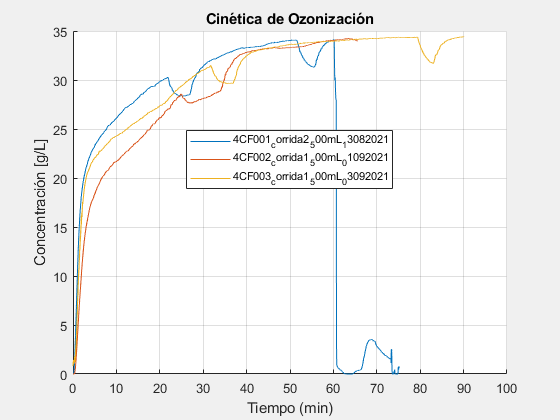
\includegraphics[width=\maxwidth{56.196688409433015em}]{figure_0.png}
\end{center}
\begin{matlaboutput}
ans = 
  laiiqatoolbox with properties:

              rawdata: {[2x498709 double]  [2x421267 double]  [2x568493 double]}
            fixeddata: {[2x450938 double]  [2x393631 double]  [2x540614 double]}
                title: "Cinética de Ozonización"
               xlabel: 'min'
                   xf: {'end'  'end'  'end'}
               ylabel: "Concentración [g/L]"
                 grid: 'on'
            LineWidth: 0.5000
               legend: {["4CF001_corrida2_500mL_13082021"]  ["4CF002_corrida1_500mL_01092021"]  ["4CF003_corrida1_500mL_03092021"]}
       legendFontSize: 8
       legendLocation: 'best'
      imageResolution: 300
     titleInterpreter: 'tex'
     labelInterpreter: 'tex'
    legendInterpreter: 'tex'
           ozoneUnits: 'g/L'
         ozoneresults: []

\end{matlaboutput}


\matlabheadingtwo{Moficación de las propiedades del objeto}

\begin{par}
\begin{flushleft}
Para modificar el titulo del gráfico:
\end{flushleft}
\end{par}

\begin{matlabcode}
miobjeto1.title = 'Mi Gráfico 1'
\end{matlabcode}
\begin{matlaboutput}
miobjeto1 = 
  laiiqatoolbox with properties:

              rawdata: {[2x498709 double]  [2x421267 double]  [2x568493 double]}
            fixeddata: {[2x450938 double]  [2x393631 double]  [2x540614 double]}
                title: 'Mi Gráfico 1'
               xlabel: 'min'
                   xf: {'end'  'end'  'end'}
               ylabel: "Concentración [g/L]"
                 grid: 'on'
            LineWidth: 0.5000
               legend: {["4CF001_corrida2_500mL_13082021"]  ["4CF002_corrida1_500mL_01092021"]  ["4CF003_corrida1_500mL_03092021"]}
       legendFontSize: 8
       legendLocation: 'best'
      imageResolution: 300
     titleInterpreter: 'tex'
     labelInterpreter: 'tex'
    legendInterpreter: 'tex'
           ozoneUnits: 'g/L'
         ozoneresults: []

\end{matlaboutput}


\matlabheadingthree{Ajuste de \textit{x }final para cada linea de datos}

\begin{par}
\begin{flushleft}
Cambiamos el valor de \textit{x }final de la primer linea de datos con la propiedad \texttt{xf:}
\end{flushleft}
\end{par}

\begin{matlabcode}
miobjeto1.xf{1} = 60 % Asignamos el valor (en unidades de tiempo) de xf para la primer linea de datos.
\end{matlabcode}
\begin{matlaboutput}
miobjeto1 = 
  laiiqatoolbox with properties:

              rawdata: {[2x498709 double]  [2x421267 double]  [2x568493 double]}
            fixeddata: {[2x450938 double]  [2x393631 double]  [2x540614 double]}
                title: 'Mi Gráfico 1'
               xlabel: 'min'
                   xf: {[60]  'end'  'end'}
               ylabel: "Concentración [g/L]"
                 grid: 'on'
            LineWidth: 0.5000
               legend: {["4CF001_corrida2_500mL_13082021"]  ["4CF002_corrida1_500mL_01092021"]  ["4CF003_corrida1_500mL_03092021"]}
       legendFontSize: 8
       legendLocation: 'best'
      imageResolution: 300
     titleInterpreter: 'tex'
     labelInterpreter: 'tex'
    legendInterpreter: 'tex'
           ozoneUnits: 'g/L'
         ozoneresults: []

\end{matlaboutput}


\begin{par}
\begin{flushleft}
Para aplicar los cambios echos a las propiedades ejecutamos el método \texttt{plotfiles} de nuevo:
\end{flushleft}
\end{par}

\begin{matlabcode}
miobjeto1.plotfiles; % Con ; evitamos mostrar las propiedades  en el Command Window
\end{matlabcode}
\begin{center}
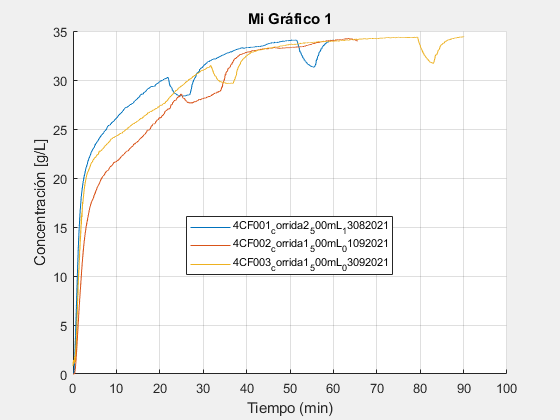
\includegraphics[width=\maxwidth{56.196688409433015em}]{figure_1.png}
\end{center}


\begin{par}
\begin{flushleft}
Cambiamos el tercer valor de \texttt{xf}:
\end{flushleft}
\end{par}

\begin{matlabcode}
miobjeto1.xf{3} = 50; % Asignamos un vamor de 50 minutos a la tercera linea de datos.
miobjeto1.plotfiles; % Aplicamos los cambiamos al gráfico.
\end{matlabcode}
\begin{center}
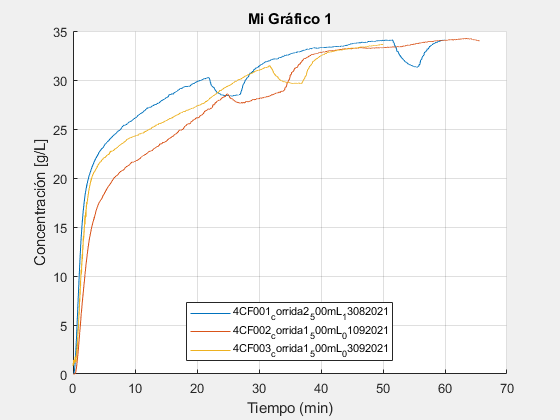
\includegraphics[width=\maxwidth{56.196688409433015em}]{figure_2.png}
\end{center}


\begin{par}
\begin{flushleft}
Para cambiar los 3 valores de \texttt{xf }al mismo tiempo:
\end{flushleft}
\end{par}

\begin{matlabcode}
miobjeto1.xf = {60 'end' 50}; % Asignamos un valor de 60 min 
% a la primer linea de datos, todos los datos a la linea 2 y 
% 50 min a la linea 3.
miobjeto1.plotfiles; % Aplicamos los cambios al gráfico.
\end{matlabcode}
\begin{center}
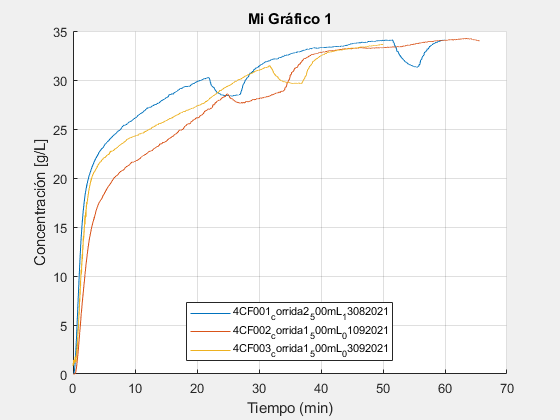
\includegraphics[width=\maxwidth{56.196688409433015em}]{figure_3.png}
\end{center}


\begin{par}
\begin{flushleft}
Quitamos el titulo del gráfico, cambiamos la etiqueta del eje \textit{y, }desactivamos las gradillas y cambiamos los nombres de las leyendas:
\end{flushleft}
\end{par}

\begin{matlabcode}
miobjeto1.title = ''; % Quitamos titulo
miobjeto1.ylabel = 'Concentración [g/Nm^3]'; % Cambio de g/L a g/Nm^3
miobjeto1.grid = 'off'; % Desactiva las rejillas
miobjeto1.legend = {'Datos Linea 1' 'Datos Linea 2' 'Datos Linea 3'}; % Renombrado de leyendas
miobjeto1.plotfiles; % Aplicamos los cambios
\end{matlabcode}
\begin{center}
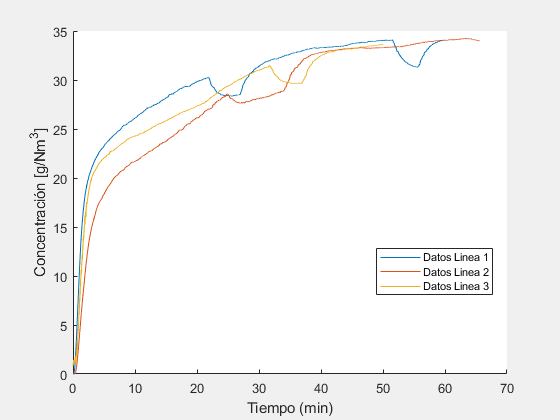
\includegraphics[width=\maxwidth{56.196688409433015em}]{figure_4.png}
\end{center}


\matlabheadingtwo{Calculo del consumo de ozono}

\begin{par}
\begin{flushleft}
Una vez ejecutados los métodos \texttt{openfiles} y \texttt{plotfiles} se puede ejecutar el método \texttt{ozonecalc}:
\end{flushleft}
\end{par}

\begin{matlabcode}
miobjeto1.ozonecalc;
\end{matlabcode}
\begin{matlaboutput}
Para Datos Linea 1:
    Consumido: 1.775 g/L
    Residual: 0.27064 g/L
    Total: 2.0456 g/L


Para Datos Linea 2:
    Consumido: 1.8347 g/L
    Residual: 0.41338 g/L
    Total: 2.2481 g/L


Para Datos Linea 3:
    Consumido: 1.3811 g/L
    Residual: 0.30163 g/L
    Total: 1.6828 g/L
\end{matlaboutput}
\begin{matlabcode}

\end{matlabcode}

\end{document}
